\documentclass[conference]{IEEEtran}
\IEEEoverridecommandlockouts
% The preceding line is only needed to identify funding in the first footnote.
% If that is unneeded, please comment it out.
\usepackage[backend=biber,style=numeric,sorting=none]{biblatex}
\usepackage{amsmath,amssymb,amsfonts}
\usepackage{algorithmic}
\usepackage{graphicx}
\usepackage{textcomp}
\usepackage{xcolor}
\addbibresource{References/article_references.bib}
\def\BibTeX{{\rm B\kern-.05em{\sc i\kern-.025em b}\kern-.08em
    T\kern-.1667em\lower.7ex\hbox{E}\kern-.125emX}}
\begin{document}

\title{Procedural generation of levels for the Angry Birds videogame using
evolutionary computation\\
}

\author{\IEEEauthorblockN{1\textsuperscript{st} Jaime Salinas-Hernández}
\IEEEauthorblockA{\textit{Department of Graduate Studies} \\
\textit{Tijuana Institute of Technology}\\
Tijuana, México \\
salinas.jaime1217@gmail.com}
\and
\IEEEauthorblockN{2\textsuperscript{nd} Mario Garcia-Valdez}
\IEEEauthorblockA{\textit{Department of Graduate Studies} \\
\textit{Tijuana Institute of Technology}\\
Tijuana, México \\
mario@tectijuana.edu.mx}
\and
\IEEEauthorblockN{3\textsuperscript{rd} Juan-J. Merelo-Guervós}
\IEEEauthorblockA{\textit{Dept. Computer Technology and Architecture} \\
\textit{University of Granada\\
Granada, Spain \\
jmerelo@ugr.es}
}

\maketitle

\begin{abstract}
% We do not say this project, is more like: In this paoer an evolutionary ... 
% is presented or In this paper we present a .... (in third or first person plural) - MG    
This project consisted in the generation of an evolutionary computation-based
system capable of generate and evolve the structures of which one level of the
Angry Birds game is composed, these structures are evaluated according to the
stability of the structure as well as for the complexity of said structure.
% This is not true any more. Also the evaluation of the level is not the most
% important aspect - MG 

A level generation system was designed based on the data obtained from
the game, said data consist in the number and type of pieces that appear and the
applied gravity of the game, proposed solutions are evaluated by a
simulation of the generated level and then checking how the structures are
affected by the gravity of the game. % This is not what the systems does any more
% It seems like you are describing Laura's work - M 

The evolutionary computation system has the main objective of generating
structures based on the existent pieces of the game and evolving said pieces by
combining them in a process that simulates the rules of the Open-Ended Evolution
algorithm in which the evolution of this compounds is not inclined towards a
numeric objective rather than to extend the diversity from which the pieces may
be selected for a level.

% The abstract is not only for stating what whas done, it is also for 
% telling readers, why they should care, what's novel, how good it is, how you tested.
% Please get some inspirtation from other abstracts on the same subject,
% this should be the last section we write. - M   
\end{abstract}

\begin{IEEEkeywords}
genetic algorithm, procedural generated content, open-ended evolution,
evolutionary computation
\end{IEEEkeywords}

\section{Introduction}
Procedural content generation is an interesting subject on the entertainment
industry, primarily in the video game development because of the easines and
quickness provided to generate content for diferent video game projects [ref] .
In this paper an evolutionary content generation system is proposed to generate
levels for the popular Angry Birds video game
\cite{RovioEntertainmentCorporation2009}, taking inspiration in concepts of
open-ended evolution.

% This paragraph is redundant only uncomment if space is abundant - M

%For this project a procedural generation content system is proposed for the game
%angly birds, angry birds is a game developed by Rovio Entrtainment in which the
%objective is to destroy structures placed on the map as well as eliminating
%green pig-like entities in order to obtain the highest score possible, the game
%mechanics is to use a slingshot to shoot a certain number of birds with
%different abilities to destroy the structures and the objectives.

% I don't think this paragraph adds much
While it is possible to create an evolutionary agent to play the levels and
obtain the best score,  the main objective of this project is to generate the
levels can ca be played by software agents or real players, the levels themselves
need to be complex in the sense that interesting structures can be created but
it has to be possible to complete in some way.

% What is the problem?
% How we solve it? (summary)   
% What is learned?

In Section 2, a background of the subjects used on this project will be
presented, this subjects, while not all being used on by different authors on
their works provide a great help on the development of the proposed system,

% Jaime, remember there is no Background need it in this type of paper 
% Maybe that will be the introduction - M

Section 3, contains a quick overview of some aspects used by different authors
in order to tackle this problem, their design and basic functionality, in
Section 4 the description of the current state of the project is explained, from
the basis of the development to the diferent menthods that have been used to
progress on the different sections of the project, 
% Normaly there is no "Future Work" section is put together with Conclusions - MG
in Section 5 we explain the
future work of the project, where we are in the development phase and how the
future implementations are to further improve the project and finally, in
Section 6 we present our conclusions
 

\section{Background}

In this Section we provide a quick overview of the literature about the areas
that provide the basis to the development of the current project, this section
is divided in three parts, the fisrt one gives us an explanation of what
procedural content generation entails, the second one provides an explanation on
genetic algorithms and how can they be used to solve optimization problems, and
finally, the third one provides us with an overview of Open-Ended Evolution and
% use just one form, I prefer with no first caps open-ended evolution and let's 
% use an abbreviation OEE - MG  
what it means to have an Open-Ended Evolutionary algorithm.

% For this conference I think we do not need to define PCG, let's think 
% every one knows what it is. - MG 

\subsection{Procedural content generation}

Procedural Content Generation (PCG) denotes the way to automatically generate
content by algorithms instead of generating the same content by manual means
such as with different personnel.

In the videogame industry many developers use a PCG style software that produces
raw images and designs used by other personnel to improve it and use it in order
to reduce the development cycles, and the productions cost. PCG as six focus
areas listed below

PCG as six focus areas listed as follows:

% Jaime, you must add references to EVERY THING READ alsewhere : 
% We do not proposed this list, please add a reference. - MG       
\begin{itemize}
    \item Level Design: This aspect involves only the design of specific
    sections of a game, primarily those in which the player is able to interact.
    \item Audio: This aspect is focused on designing soundtracks that are able
    to react to a player specific action.
    \item Visuals: This area is focused on creating or improving visual
    representations of objects on games such as giving raw designs of players
    faces of improving the images of other graphics.
    \item Narrative: This aspect is focused on the generation of readable and
    coherent stories or plotlines of games.
    \item Gameplay: This aspect uses agents to test and evaluate the mechanic on
    which a game is based by trying to play as a human would in order to improve
    said mechanics.
    \item Game Design: This aspect is focused on generating the rulesets and mechanics of a new game. \cite{Yannakakis2017}
\end{itemize}

\subsection{Genetic algorithm}
Is a method developed by John Holland on 1975 \cite{Holland1975} % Yes ! like this - MG
the genetic
algorithm (GA) is an optimization and search technique based on the principles
of genetic and natural selection, it allows a population composed of many
individuals, which by themselves represent a possible solution to the problem,
to evolve under specific selection rules in order to obtain the maximum fitness.

In other words a genetic algorithm is a method to solve optimization problems by
creating a population that will represent a possible solution and repeatedly
doing genetic operations as selection, crossover and mutation on each member of
the population in order to generate the members of the population for the next
generation that would be closer to the best solution of the problem than their
parents, the cycles in this method where the operations are made are called
generations and by moving over this the population “evolves” o in other words,
they get closer to the best possible solution  to a specific problem.

\begin{figure}[htbp]
\centerline{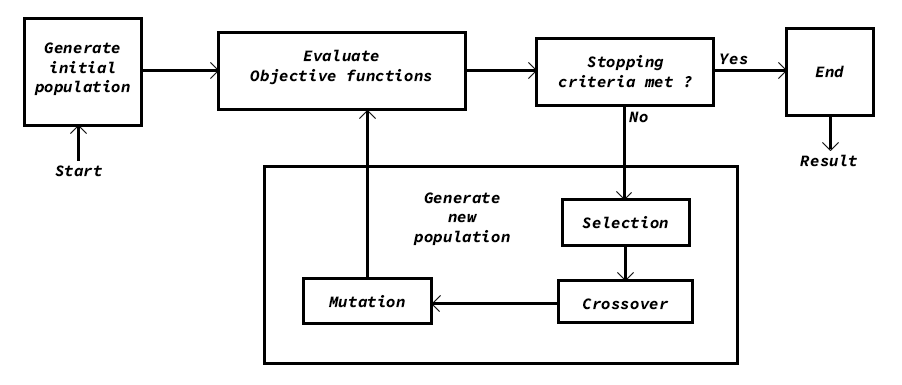
\includegraphics[width=90mm]{Images/ga_life_cycle.png}}
\caption{Life cycle of a genetic algorithm.}
\label{fig}
\end{figure}

% Maybe this is well known, again our implementation is what we need to describe 
% JJ, what you think?  

The main life cycle of a genetic algorithm shown of figure 1 is described as
follows:
\begin{enumerate}
    \item Initialize a random n population of values suitable for the solution.
    \item Evaluate the fitness of each individual (solution) in the population.
    \item Check if the stopping criteria has been met.
    \item If not.
    \begin{enumerate}
        \item Introduce new individuals to the population by crossover
        operations.
        \item Mutate a random value of the new individuals.
        \item Select new cross over individuals according to their fitness for
        the next generation.
    \end{enumerate}
    \item Loop from step 2 until an end condition is satisfied.
    \item Select the best individual of the population as the solution for the
    problem
\end{enumerate}

% This section and the proposed approach should be in the fron lines - MG

% The problem is that we just state what it is, but we do not link it
% with our work. Why is important? What inpired our work? 
% There is also Novelty Search - MG
% Also it sounds like a copy-paste from Wikipedia please check and reference
% accordingly - MG

\subsection{Open-Ended Evolution}\label{AA} 
Open-ended evolution (OEE) is a variant of genetic evolution algorithm in which
the objective differs from the regular genetic algorithm one, in this case the
final objective is not to reach a final state of the evolution but to continue
evolving and creating new types of entities more complex on each new generation,
these same entities have the possibility to evolve not only inside the frame of
their type but create entirely new groups. \cite{Standish2003}

Another explanation provided by T. Taylor et al. \cite{Taylor2016} defines OEE
has a system capable of creating novelty beyond a point where nothing changes on
the current group of interest rather than just converging to a stable or
quasi-stable state.

For this project OEE is defined simply has a process of genetic evolution that
encapsulates a group of similar processes and that is able to increase their
number by the more complex the entities become.

\section{Overview of existing work}

In this Section we present some of the different approaches to the procedural
generation of content for the angry birds video game.

M. Kaidan et al. \cite{Kaidan2015} propose a model in which the generation of
content is controlled by the skill of a player while actively playing the game,
the moment the player finishes a certain level the algorithm obtains the score
and generates the next level to be played.

J. Renz et al. \cite{Renz} created an article in which the angry birds level
generation contest mechanics of the IEEE Conference on Computational
Intelligence and Games are based on, it explains some of the solving methods
proposed by previous competitors.

Y. Jiang et al. \cite{Jiang2017} proposed the use of predefined letter style
patterns and combined the to create a small pool of word used to be combined in
order to create levels with text on them, the participants would play the game
and after that they would be asked if they liked the layout of the levels

\section{Current approach}

In this Section we describe the approach that was used for this project, The
game contains a total of 11 pieces as shown on figure 2 that cannot be modified,
it is not possible to add more or modify the existing ones, with this in mind
the purpose is to create bundles of this same pieces in different locations and
angles in order to create structures that can be used as building blocks for
more complex levels, in order to do this a sequence of events needs to be done
as follows:

% Pleas explain in more detail this Composites in a section.  

% Please use the name Composite instead of Bundle, composition is well known in
% object oriented design.

\begin{enumerate}
\item Generate the first generation of the population
\item Run a Simulation
\item Evaluate each member of the population
\item If a member of the population has remaining pieces obtain the location and
angle of the pieces, create a bundle and add it to the pool
\item Select the parents for the next generation
\item Do the crossover and mutation operations
\item Repeat the cycle
\end{enumerate}

\begin{figure}[htbp]
\centerline{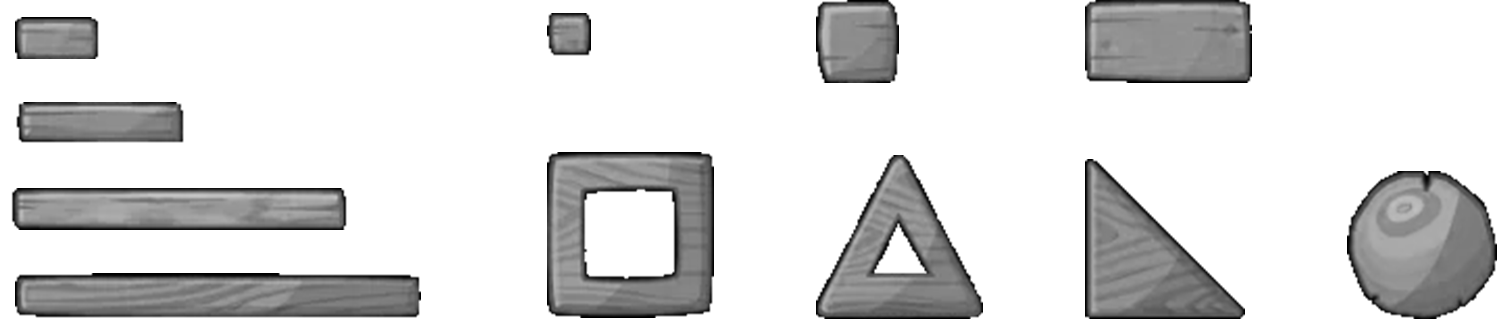
\includegraphics[width=80mm]{Images/list_pieces.png}}
\caption{List of pieces in the angry birds game.}
\label{fig}
\end{figure}

% This sentence needs more work -MG
Since the algorithm has to generate more complex structures the remaining
pieces of a member of the population have to be used has a starting point, this
% we don't use member of the populations, use proposed solution, candidate solution
% or individual of the population. - MG  
new additions to the piece pool are added to the population by the mutation
operation, the objective in the first phase of the project is to generate
structures that are capable of maintaining their own balance as shown on figure
3, since the objective of open-ended evolution for this project is to add new
bundles to the pool of options the algorithm will first run a simulation with a
group of pieces and after it the ones that were not destroyed by falling because
of gravity will be saved and added to the pool of options.

% New pieces are added by mutation? 
% Please give more details to all this - MG

\begin{figure}[htbp]
\centerline{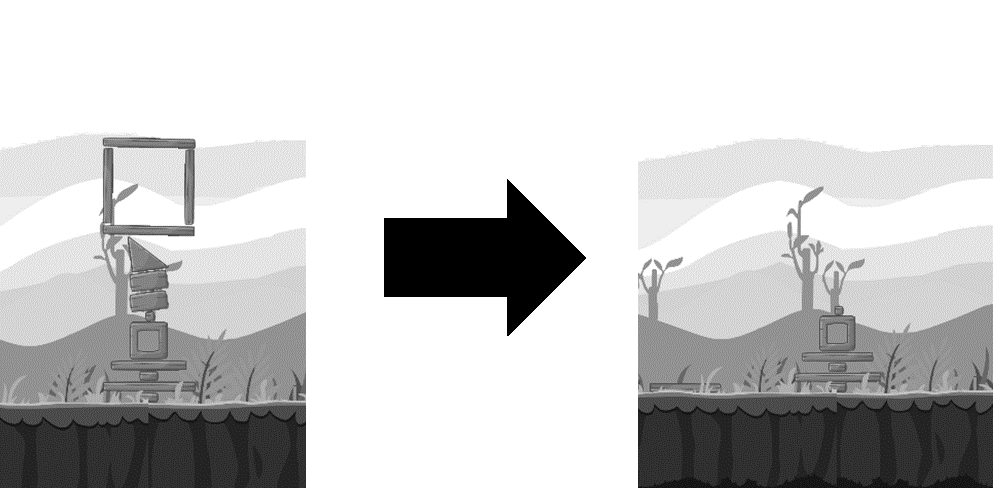
\includegraphics[width=80mm]{Images/simulation_bef_aft_example.png}}
\caption{Structure at beginning and end of a simulation.}
\label{fig}
\end{figure}

% Here it's explained better, maybe this paragraph should be moved to
% an earlier point - MG

% Needs a few touches - MG

In order to add a bundle of pieces as a new component first it has to be
measured, an imaginary bounding box is defined by calculating the lengths of all
the pieces, finding the borders of said pieces and find the points that could
define a box around all of them, calculate the height and width then calculate
the center point of said box and calculate the offsets from the center of the
group to the center of each respective piece as shown on figure 4, this
information is needed in order to add it as a new element so it can be used to
place the pieces in their respective new positions when the files needed for the
simulation are being created.

The way to represent the elements of a member of the population is by using the
id of each piece and the new added ones has a pointer to the respective data
that needs to be obtained, this way and individual can be represented as shown
on figure 5 where each chromosome represents a certain item in the pool of
pieces, the numbers for this elements are assigned in a first come first served
basis, the numbers are infinitely incremented and this same pieces can be
repeated on each individual of the population

\begin{figure}[htbp]
\centerline{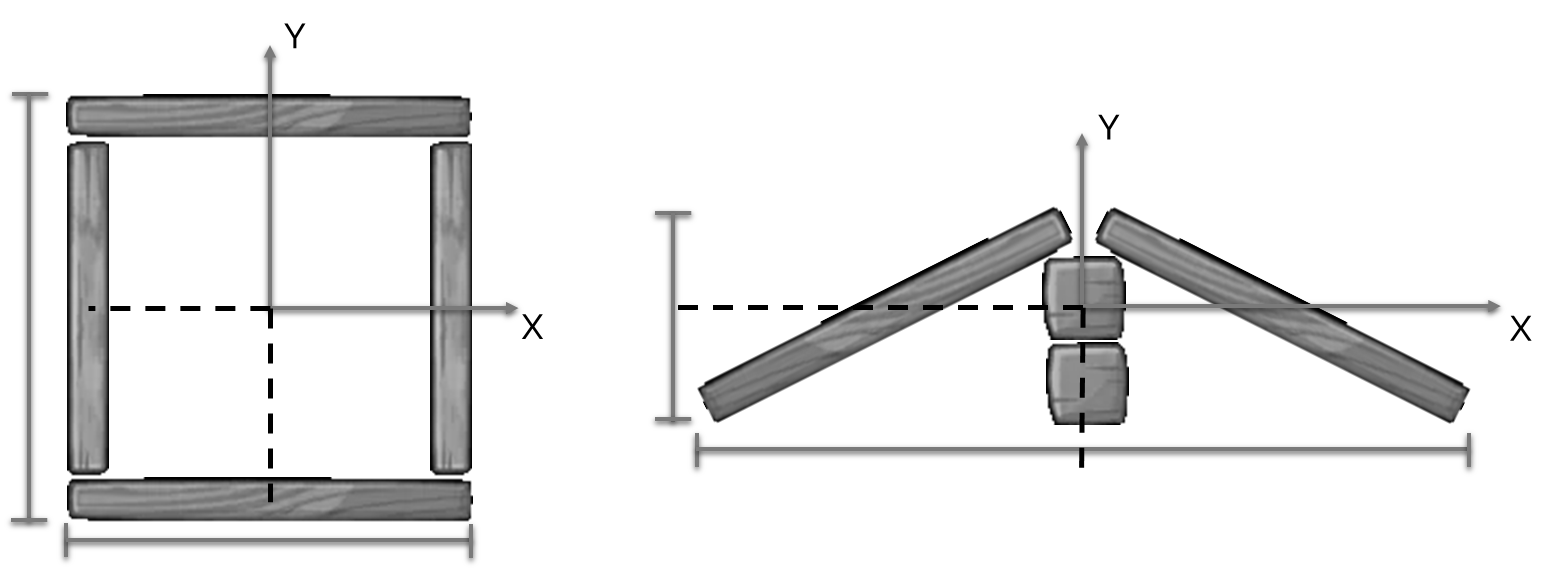
\includegraphics[width=80mm]{Images/bounding_box_calculation.png}}
\caption{bounding box calculation.}
\label{fig}
\end{figure}

\begin{figure}[htbp]
\centerline{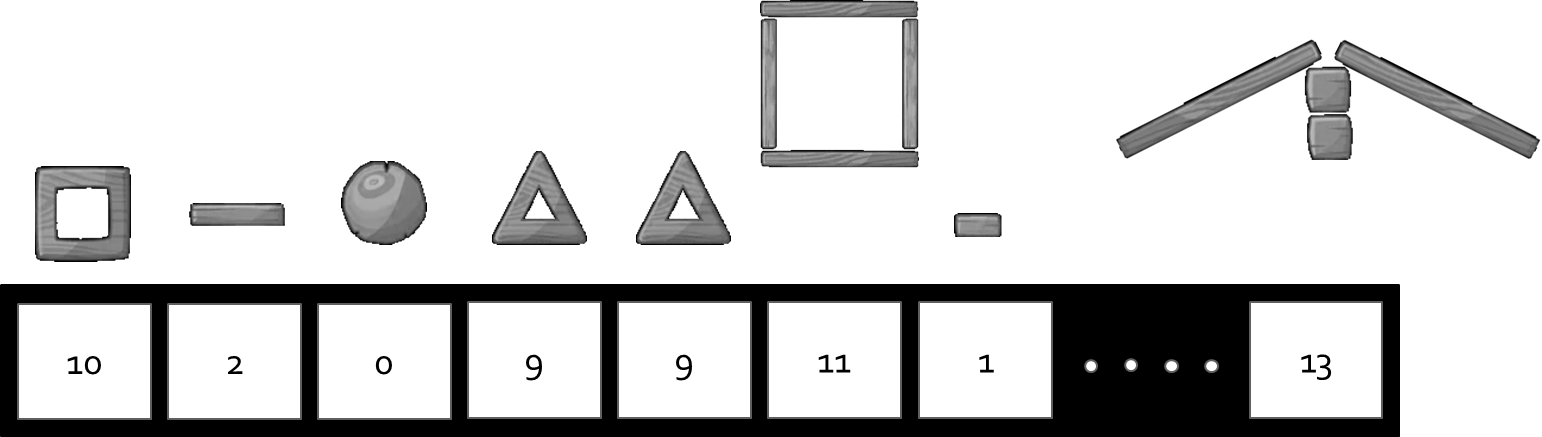
\includegraphics[width=80mm]{Images/chromosome_chain_example.png}}
\caption{Chromosome chain of an individual.}
\label{fig}
\end{figure}

Once the pieces have been added and the individuals are ready to be evaluated a
simulation on the game environment is scheduled by order in the population, all
the individuals have a maximum of ten seconds to maintain balance or reach
absolute stability, if absolute stability is reached it means one of two things,
first the generated structure is completely stable or second, the tower fell to
either side and the pieces were destroyed or stopped moving by gravitational
pull, when either of this happens by more than two seconds the simulation ends
regardless of time remaining and the next individual is simulated.

The evaluation process for this project is still in the development stages,
however in order to check that the evolution is working has it should a criteria
has been temporarily made as follows, each individual in the population has 100
points so before the simulation starts each of them are viable candidates to be
a elite member of the population regardless relative height or complexity, then
the remaining of the process is separated in three phases has follows.

First, after each of the individual simulations are over the evaluation process
takes place, in this phase the resulting level is checked for pieces, each one
of them is counted and then the resulting number is compared to that of the
initial quantity of pieces that were originally put in before the simulation in
order to calculate the first element of the evaluation process, each piece
represents a certain percentage of 100\% so the missing pieces are subtracted
from the total.

Second, after removing percentage according to the missing pieces an individual
remaining pieces are checked for their positions in comparison to the original
ones before the simulation, using the formula 1 each piece within the individual
is evaluated according to the center point of the piece, if the piece moved more
than a certain threshold half the percentage for one piece is removed from the
remaining percentage, after this using the formula 2 the position of the piece
is further checked this time by the difference in angle from the original one,
in case the difference of angles is more than a certain threshold half a piece
value is further removed from the total.

\begin{equation}
    \begin{aligned}
    error_{xy} = \left\{ \,
        \begin{IEEEeqnarraybox}[][c]{l?s}
            \IEEEstrut
            0.1 & if $ 0.08 > d $, \\
            \frac{100}{lenght\_pieces} * 0.5 & if $ 0.08 < d $.
            \IEEEstrut
        \end{IEEEeqnarraybox}
    \right. \\
    where: d=\sqrt{(x_2 - x_1)^2 + (y_2 - y_1)^2}    
    \end{aligned}
\end{equation}

\begin{equation}
    \begin{aligned}
    error_{r} = \left\{ \,
        \begin{IEEEeqnarraybox}[][c]{l?s}
            \IEEEstrut
            0 & if $ -5 \le r \le 5 $, \\
            \frac{100}{lenght\_pieces} * 0.5 & if $ r < 5 or r > 5 $.
            \IEEEstrut
        \end{IEEEeqnarraybox}
    \right. \\
    where: r= |rotation_0| - |rotation_f|   
    \end{aligned}
\end{equation}

Finally, the total height of the remaining group of pieces is calculated by
combining the bonding boxes of all pieces, then the individuals are ordered by
the obtained percentage and then further ordered by the total height, this way
the most balanced ones will have the best probability to be selected together
for a crossover operation to create the next generation.

\begin{figure}[htbp]
\centerline{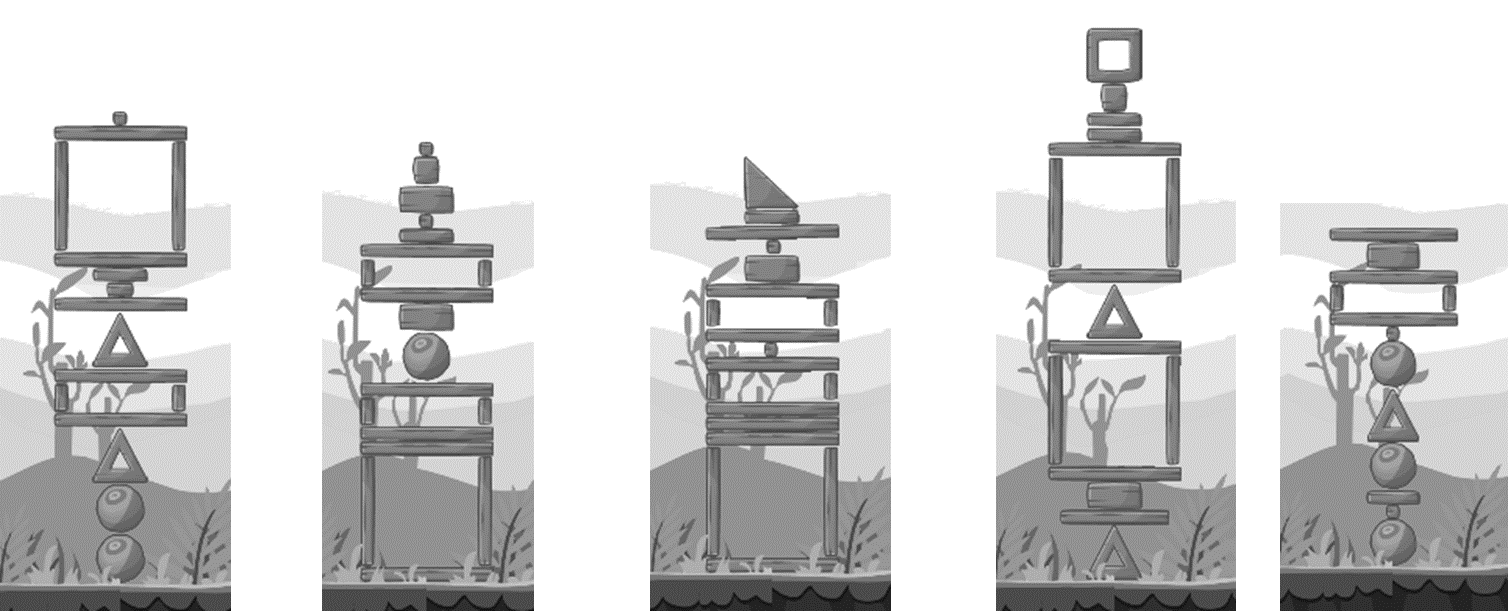
\includegraphics[width=80mm]{Images/result_example.png}}
\caption{Result samples of current system.}
\label{fig}
\end{figure}

\section{Future work}
Since there is a need to create complex structures than can cover a great
section of the play map, a method to evaluate the distribution is needed, for
this instance we propose using the rule of thirds \cite{DarrenRowse} which is a
guideline used while creating imagen in which the purpose is to create
aesthetical pleasant images where the focus point or the most important area is
at the center of the image as shown on figure 7, using this rule different
distribution groups or masks are created has shown on figure 8 in order to use
them before the simulation of an individual takes place in order to distribute
the pieces in a way that can cover more area and create more balanced levels
instead of using a tower like distribution as shown on figure 9. Using this same
distribution a new evaluation will be added in which according to how much of
the area is filled a score will be given and this score will be used as a new
sorting value at the moment of selecting individuals for the crossover
operation, since as shown on figure 8 there is a possibility that a huge mask is
given to an individual it can be possible that the amount of pieces will not be
able to cover the full area given, so in order to prevent this kind of problems
we also propose to give each mask a value that refers to the minimum amount of
pieces and height required to fill the most of the mask then check the amount of
pieces and height before simulation for a single individual and then randomize
which mask of the ones that can be used will be assigned to that individual

\begin{figure}[htbp]
    \centerline{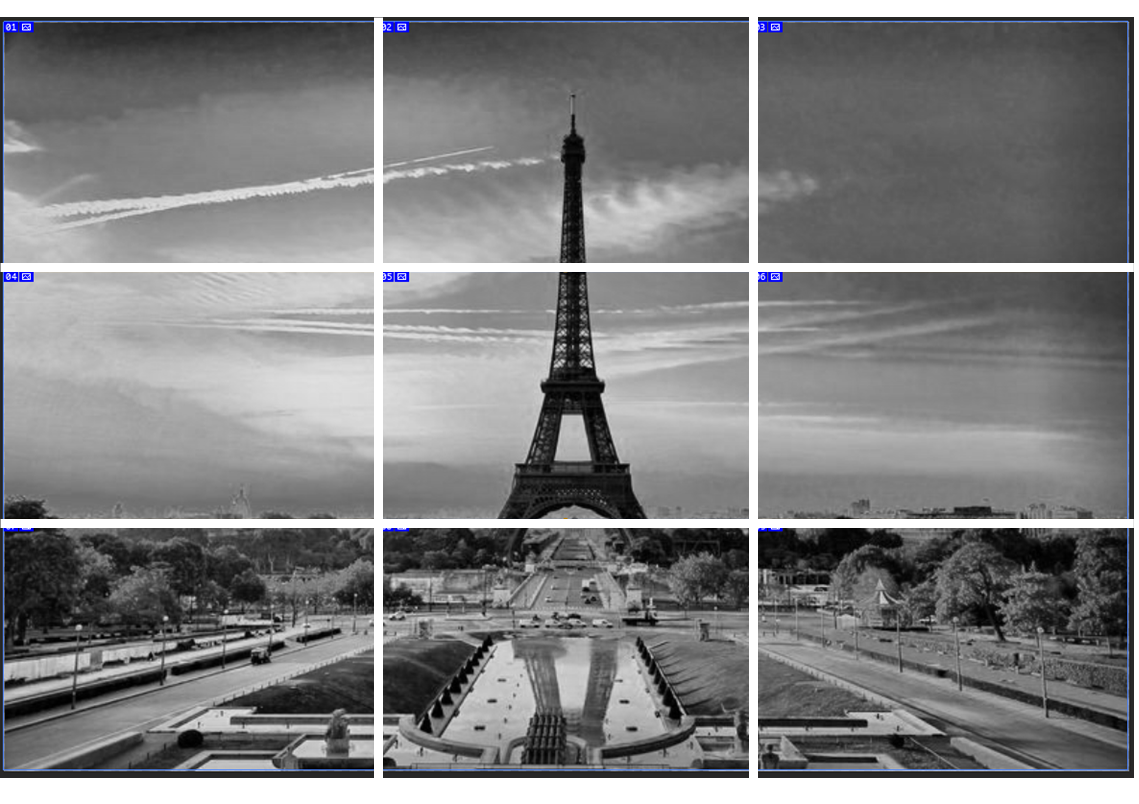
\includegraphics[width=80mm]{Images/ruleofthirds_example.png}}
    \caption{Rule of thirds example.}
    \label{fig}
\end{figure}

\begin{figure}[htbp]
    \centerline{
\includegraphics[width=80mm]{Images/mask_distribution.png}}
    \caption{Rule of thirds applied to an individual.}
    \label{fig}
\end{figure}

\section{Conclusions}

The use of artificial intelligence in videogames is a common thing almost since
before the first generation of videogames on 1972 as simply entities that would
follow a set group of actions but as the generation kept advancing the need for
more intelligent entities appeared, as of this generation some videogames use AI
as ways to improve the interaction between man and game, but also using it in
order to facilitate the way videogames are created, so for this project the
focus of using evolutionary algorithms as great interest, as a starting point a
rather simple game can be used as a workbench of the work but it also helps us
define how much more can be done when all the required objects are obtained,
improve on the same system and find ways for it to be used on different other
games

\printbibliography
\newrefcontext[sorting=ydnt]

\end{document}
